\documentclass[
]{jdssv}

%% recommended packages
\usepackage{orcidlink,thumbpdf,lmodern}

\usepackage[utf8]{inputenc}

\author{
Patrick J.F. Groenen\\Erasmus University Rotterdam \And Stefan Van
Aelst\\KU Leuven
}
\title{Guidelines for the Journal of Data Science, Statistics, and
Visualisation}

\Plainauthor{Patrick J.F. Groenen, Stefan Van Aelst}
\Plaintitle{Guidelines for the Journal of Data Science, Statistics, and
Visualisation Version 0.3}
\Shorttitle{JDSSV Guidelines, Version 0.3}


\Abstract{
This short article illustrates how to write a manuscript for the
\emph{Journal of Data Science, Statistics and Visualisation} (JDSSV)
using its \LaTeX~style files. Please follow JDSSV's style guidelines
precisely. Also, it is recommended to keep the \LaTeX~code as simple as
possible, that is, avoid inclusion of packages/commands that are not
necessary.
}

\Keywords{JDSSV, style guidelines, comma-separated, not
capitalized, \proglang{R}}
\Plainkeywords{JDSSV, style guidelines, comma-separated, not
capitalized, R}

%% publication information
%% \Volume{50}
%% \Issue{9}
%% \Month{June}
%% \Year{2012}
%% \Submitdate{}
%% \Acceptdate{2012-06-04}

\Address{
    Patrick J.F. Groenen\\
    Erasmus University Rotterdam\\
    Econometric Institute\\
Erasmus School of Economics\\
Erasmus University Rotterdam\\
P.O. Box 1738\\
3000 DR Rotterdam, The Netherlands\\
  E-mail: \email{groenen@ese.eur.nl}\\
  URL: \url{https://personal.eur.nl/groenen/}\\~\\
      Stefan Van Aelst\\
    KU Leuven\\
    ~Department of Mathematics\\
\hspace*{0.333em}KU Leuven\\
\hspace*{0.333em}Celestijnenlaan 200B\\
\hspace*{0.333em}3001 Leuven, Belgium\\
  E-mail: \email{Stefan.VanAelst@kuleuven.be}\\
  URL: \url{https://wis.kuleuven.be/statdatascience/robust}\\~\\
  }


% tightlist command for lists without linebreak
\providecommand{\tightlist}{%
  \setlength{\itemsep}{0pt}\setlength{\parskip}{0pt}}




\usepackage{amsmath} \usepackage{longtable} \usepackage{booktabs} \newcommand{\class}[1]{`\code{#1}'} \newcommand{\fct}[1]{\code{#1()}} \newcommand{\ma}[1]{\ensuremath{\mathbf{#1}}}

\begin{document}



\hypertarget{mission}{%
\section{Mission}\label{mission}}

JDSSV\footnote{This document is an adaptation of the style guide of the Journal of Statistical Software \citep{jss_style_guide}.}
is an international refereed journal that creates a forum to present
recent progress and ideas in the different disciplines of data science,
statistics, and visualisation. It welcomes contributions to data
science, statistics, and visualisation, and in particular those aspects
which link and integrate these subject areas. Articles can cover topics
such as machine learning and statistical learning, the visualisation and
verbalisation of data, visual analytics, big data infrastructures and
analytics, interactive learning, and advanced computing. Papers that
discuss two or more research areas of the journal are favoured.
Scientific contributions should be of a high standard. Articles should
be oriented towards a wide scientific audience of statisticians, data
scientists, computer scientists, data analysts, etc.

The journal welcomes original contributions that are not being
considered for publication elsewhere and contain a high level of
novelty. Papers with a thorough but concise review of a certain topic
with the potential to provide new insights are also welcome. Manuscripts
submitted to the journal generally are accompanied by supplementary
material that containing software code, technical derivations or
detailed explanations, additional examples, etc. All submitted material
will be reviewed by the assigned associate editor and reviewers of the
manuscript.

Manuscripts may have a substantial theoretical component, but it is
expected that all manuscripts contain at least one application on
empirical or simulated data. The journal emphasizes the reproducibility
of the results presented its papers. Therefore, all data and software
code that is necessary to reproduce the empirical results in the
manuscript should be made available in a user friendly manner. If the
empirical data cannot be released for reasons of confidentiality or
otherwise, then a generated dataset with comparable properties should be
provided.

\hypertarget{preparing-your-manuscript-for-submission}{%
\section{Preparing your Manuscript for
Submission}\label{preparing-your-manuscript-for-submission}}

All submissions to JDSSV should be written in \LaTeX~using the JDSSV
style files provided on the journal website \url{https://jdssv.org}. For
initial submission it suffices providing the pdf version of the
manuscript together with all the necessary supplementary material
including software code to reproduce all results in the manuscript. The
final version of accepted manuscripts should adhere to all the style
guidelines and should incorporate all changes requested by the
production editor. All \LaTeX~ source files of the final manuscript
should be submitted and accepted manuscripts are only published if these
files comply with all guidelines and instructions provided by the
journal.

\hypertarget{software}{%
\section{Software}\label{software}}

The journal expects that submissions contain accompanying software with
the aim of reproducibility of the results and application of the
proposed methodology to other data by the reader. All existing software
used in the paper should be properly referenced. Code should be
delivered in an easily readable manner with clear instructions on its
use, and preferably is accompanied by instructive examples of its use.
We highly recommend to provide code that can be used in open-source
software such as \proglang{R} \citep{R}, \proglang{Python}
\citep{python}, \proglang{Julia} \citep{Julia}, \proglang{Octave}
\citep{octave}, etc.

To make code widely accessible, we advise making it available in a
repository such as \url{https://zenodo.org} where it will receive a
permanent Digital Object Identifier (DOI) which can be included in the
manuscript.

The provided code should at least consist of a file or set of files for
the functions that execute the core of the method. For reproducibility,
another necessary file is the script that creates the results (tables
and figures) of the paper. For methods that run very long, provide a toy
example that runs sufficiently fast and highlights the properties of the
method. Nonproprietary data should be provided or a permanent link to
these data should be given. The corresponding script to analyze the data
should read these data.

\begin{sloppypar}
For increased readability, please apply the following naming conventions for code: Start function names with a verb, e.g., \code{set_initialisation()}, \code{compute_loss()}, \code{update_X()}, etc. when appropriate. Give  objects descriptive names or closely follow the notation in the paper.
For programming conventions (particularly in \proglang{R}), see Hadley Wickham's guidelines (\url{http://r-pkgs.had.co.nz/style.html}) and the use of the \pkg{styler} package is recommended. For \proglang{python}, consider Google's recommendations (\url{https://github.com/google/styleguide/blob/gh-pages/pyguide.md}) Sufficient comments should be added to the code to make it understandable. For \proglang{Octave} and \proglang{MatLab} \citep{matlab}, consider Richard Johnson's MatLab Style Guidelines 2.0 (\url{https://www.mathworks.com/matlabcentral/fileexchange/46056-matlab-style-guidelines-2-0}).
\end{sloppypar}

For writing about software JDSSV requires authors to use the markup
\verb|\proglang{}| (programming languages and large programmable
systems), \verb|\pkg{}| (software packages), \verb|\code{}| (functions,
commands, arguments, etc.). If there is such markup in (sub)section
titles (as above), a plain text version has to be provided in the
\LaTeX~command as well. Below we also illustrate how abbrevations should
be introduced and citation commands can be employed. See the \LaTeX~code
for more details.

\hypertarget{review-process}{%
\section{Review Process}\label{review-process}}

All manuscripts should be submitted online at \url{https://jdssv.org}.
JDSSV uses a single blind review process. Upon submission of their
manuscript, authors have the opportunity to provide a short list of
suggested reviewers as well as a few names of researchers that
preferably should not be contacted for reviewing the manuscript. All
submitted manuscript will undergo automatic checking for plagiarism and
will not be considered for further review in case of plagiarism. The
manuscript will be assigned to one of the editors who will make an
initial screening to check the quality of the submitted work, possibly
with the help of an associate editor. After positive screening, the
manuscript will be assigned to an associate editor who will seek the
opinion of at least two reviewers. Reviewers are asked to send their
report within one month. Associate editors should typically make their
recommendation one week after reception of the review reports. The
initial review process should normally not take more than three months.
All communication between the authors and the journal will be
administered by the journal editors.

\hypertarget{sec:models}{%
\section{Correspondence Analysis}\label{sec:models}}

As an example, we provide a simple implementation of correspondence
analysis \citep[see, e.g.,][]{greenacre2010biplots}. For the analysis of
bivariate categorical data or other tables that contain counts,
correspondence analysis can be a useful technique to visualize important
relations between the categories. Consider word count data on
explanations of data science by several websources provided by
\citet{Lubbe2018}, see Table \ref{tab:word_counts}.

\begin{table}
\caption{Part of the table with word counts describing data science by different web sources as collected by \citet{Lubbe2018}.}
\label{tab:word_counts}
\begin{center}
\begin{tabular}{lccccccc} \hline
            & dsc.test & dsctechniques & datadiversity & dsc.tips & $\ldots$ & wikipedia \\ \hline
statistics  &       6  &           2   &          2    &    0     & $\ldots$ &  2 \\
big data    &       2  &           0   &          3    &    5     & $\ldots$ &  0 \\
analytics   &       1  &           0   &          2    &    0     & $\ldots$ &  2 \\
database    &       2  &           0   &          0    &    2     & $\ldots$ &  1 \\
insight     &       0  &           0   &          4    &    0     & $\ldots$ &  2 \\
$\vdots$    & $\vdots$ &    $\vdots$   &   $\vdots$    & $\vdots$ &$ \ddots$ & $\vdots$ \\
programming &       7  &           0   &          0    &    0     & $\ldots$ &  0 \\
\hline
\end{tabular}
\end{center}
\end{table}

Let \(\ensuremath{\mathbf{F}}\) be the matrix containing the values in
Table \ref{tab:word_counts}. The most simple model to fit such a table
is the independence model in matrix \(\ensuremath{\mathbf{E}}\) defined
as \begin{eqnarray*}
  \ensuremath{\mathbf{E}} = n^{-1}\ensuremath{\mathbf{D}}_r \ensuremath{\mathbf{11}}^\top \ensuremath{\mathbf{D}}_c
\end{eqnarray*} with \(\ensuremath{\mathbf{1}}\) a vector of ones of
appropriate length,
\(\ensuremath{\mathbf{D}}_r = \textrm{Diag}(\ensuremath{\mathbf{F1}})\)
the diagonal matrix with row sums of \(\ensuremath{\mathbf{F}}\),
\(\ensuremath{\mathbf{D}}_c = \textrm{Diag}(\ensuremath{\mathbf{F^\top 1}})\)
the diagonal matrix with column sums of \(\ensuremath{\mathbf{F}}\), and
\(n = \ensuremath{\mathbf{1^\top F1}}\) be the sum of all elements in
\(\ensuremath{\mathbf{F}}\). The goal of correspondence analysis is to
find a matrices of row and column coordinates
\(\ensuremath{\mathbf{R}}\) and \(\ensuremath{\mathbf{C}}\) such that
\begin{eqnarray*}
  L(\ensuremath{\mathbf{R}}, \ensuremath{\mathbf{C}}) = \|\ensuremath{\mathbf{D}}_r^{-1/2} (\ensuremath{\mathbf{F}} - \ensuremath{\mathbf{E}} - \ensuremath{\mathbf{D}}_r\ensuremath{\mathbf{RC}}\ensuremath{\mathbf{D}}_c^\top) \ensuremath{\mathbf{D}}_c^{-1/2}\|^2
\end{eqnarray*} is minimized
\citep[see, for example,][]{vandeveldenetal2009seriation}. It may be
verified that the least-squares optimal solution is obtained by
computing the singular value decomposition (SVD) \begin{eqnarray*}
  \ensuremath{\mathbf{D}}_r^{-1/2} (\ensuremath{\mathbf{F}} - \ensuremath{\mathbf{E}})\ensuremath{\mathbf{D}}_c^{-1/2} = \ensuremath{\mathbf{UDV}}^\top
\end{eqnarray*} and computing \begin{eqnarray*}
  \ensuremath{\mathbf{R}} &=& n^{1/2}\ensuremath{\mathbf{D}}_r^{-1/2} \ensuremath{\mathbf{UD}}^{\alpha}\\
  \ensuremath{\mathbf{C}} &=& n^{1/2}\ensuremath{\mathbf{D}}_c^{-1/2} \ensuremath{\mathbf{VD}}^{1-\alpha}
\end{eqnarray*} for some \(\alpha\). Note that the least-squares optimal
rank \(p\) solution is obtained by taking the first \(p\) columns of
\(\ensuremath{\mathbf{R}}\) and \(\ensuremath{\mathbf{C}}\). If
\(\alpha = 1\) the so-called row principal solution is obtained where
the row points are the weighted centroids of the column points,
\(\alpha = 0\) gives the column principal solution with column points
being the weighted average of the row points, and \(\alpha = 1/2\)
results in the symmetric solution. The importance measure of the
dimensions are given by the inertia, that is, the diagonal elements of
\(\ensuremath{\mathbf{D}}^2\). For more details, see, for example,
\cite{greenacre2010biplots}.

A simple implementation of correspondence analysis in \proglang{R} is
given by the function \code{corana()} given by

\begin{CodeChunk}
\begin{CodeInput}
R> corana <- function(dat, alpha = 0.5){
+   # Perform correspondence analysis
+   # Input: 
+   ##  dat   numeric matrix dat with nonnegative entries
+   ##  alpha = 1 is row principal standardisation
+   ##        = 0 is column principle standardisation
+   ##        = 0.5 is symmetric standardisation
+   dat <- as.matrix(dat)
+   Dr <- rowSums(dat)
+   Dc <- colSums(dat)
+   n  <- sum(Dr)
+   # Compute expected values under the independence model
+   E  <- outer(Dr, Dc)/n
+   tt <- svd(diag(Dr^-0.5) %*% (dat - E) %*% diag(Dc^-0.5))
+   ## Remove dimensions with singular value zero
+   ind <- tt$d > 1e-10
+   tt$d <- tt$d[ind]
+   tt$u <- tt$u[, ind]
+   tt$v <- tt$v[, ind]
+   ## Compute row scores R and column scores C 
+   R  <- n^0.5 * diag(Dr^-0.5) %*% tt$u %*% diag(tt$d^alpha)
+   C  <- n^0.5 * diag(Dc^-0.5) %*% tt$v %*% diag(tt$d^(1 - alpha))
+   rownames(R) <- rownames(dat)
+   rownames(C) <- colnames(dat)
+   ## Compute relative contribution to inertia per dimension 
+   row.inert   <- outer(Dr/n, tt$d^(2*alpha),       "/") * R^2
+   col.inert   <- outer(Dc/n, tt$d^(2*(1 - alpha)), "/") * C^2
+   ## Compute reconstructed Chi-square distance for row and column points
+   row.dist    <- R^2 %*% diag(tt$d^(2 - 2*alpha))
+   row.dist    <- row.dist / outer(rowSums(row.dist), rep(1, ncol(R))) 
+   col.dist    <- C^2 %*% diag(tt$d^(2 - 2*(1 - alpha)))
+   col.dist    <- col.dist / outer(rowSums(col.dist), rep(1, ncol(C))) 
+   ## Prepare list of results
+   out <- list(R = R, C = C, sing.val = tt$d, 
+               row.inert = row.inert, col.inert = col.inert,
+               row.dist  = row.dist,  col.dist  = col.dist)
+   class(out) <- "corana"
+   return(out)
+ }
\end{CodeInput}
\end{CodeChunk}

A plot is given by the \code{plot.corana()} method

\begin{CodeChunk}
\begin{CodeInput}
R> plot.corana <- function(out, dims = 1:2, ...){
+   R <- out$R[, dims]
+   C <- out$C[, dims]
+   ## Set up coordinate system
+   coord <- rbind(R, C)
+   plot(coord[, 1], coord[, 2], type = "n", asp = 1, las = 1,
+        xlab = paste0("Dim ", dims[1]), ylab = paste0("Dim ", dims[2]), ...)
+   abline(h = 0, v = 0, col = "gray")
+   ## Use reconstructed distance as importance measure for transparency and size
+   row.alpha <- rowSums(out$row.dist[, dims])
+   row.alpha <- (row.alpha/max(row.alpha))^0.7
+   col.alpha <- rowSums(out$col.dist[, dims])
+   col.alpha <- (col.alpha/max(col.alpha))^0.7
+   ## Plot row and column points 
+   points(R[, 1], R[, 2], pch = 20, col = rgb(1, 0, 0, row.alpha))
+   points(C[, 1], C[, 2], pch = 20, col = rgb(0, 0, 1, col.alpha))
+   ## Write text labels
+   text(R[, 1], R[, 2], rownames(R), pos = compute.pos(R), cex = 2*row.alpha,
+        col = rgb(1, 0, 0, ifelse(row.alpha > 0.1, row.alpha, 0)))
+   text(C[, 1], C[, 2], rownames(C), pos = compute.pos(R), cex = 2*col.alpha,
+        col = rgb(0, 0, 1, ifelse(col.alpha > 0.1, col.alpha, 0)))
+ }
\end{CodeInput}
\end{CodeChunk}

Assuming that \code{ds.word.cnt} contains the full matrix of which a
part is shown in Table \ref*{tab:word_counts}, then the following code
does a correspondence analysis on these data:

\begin{CodeChunk}
\begin{CodeInput}
R> load("ds.word.cnt.RData")
R> source("compute.pos.R")
R> out.corana <- corana(ds.word.cnt)
R> plot(out.corana, dims = 2:3)
\end{CodeInput}
\begin{figure}

{\centering 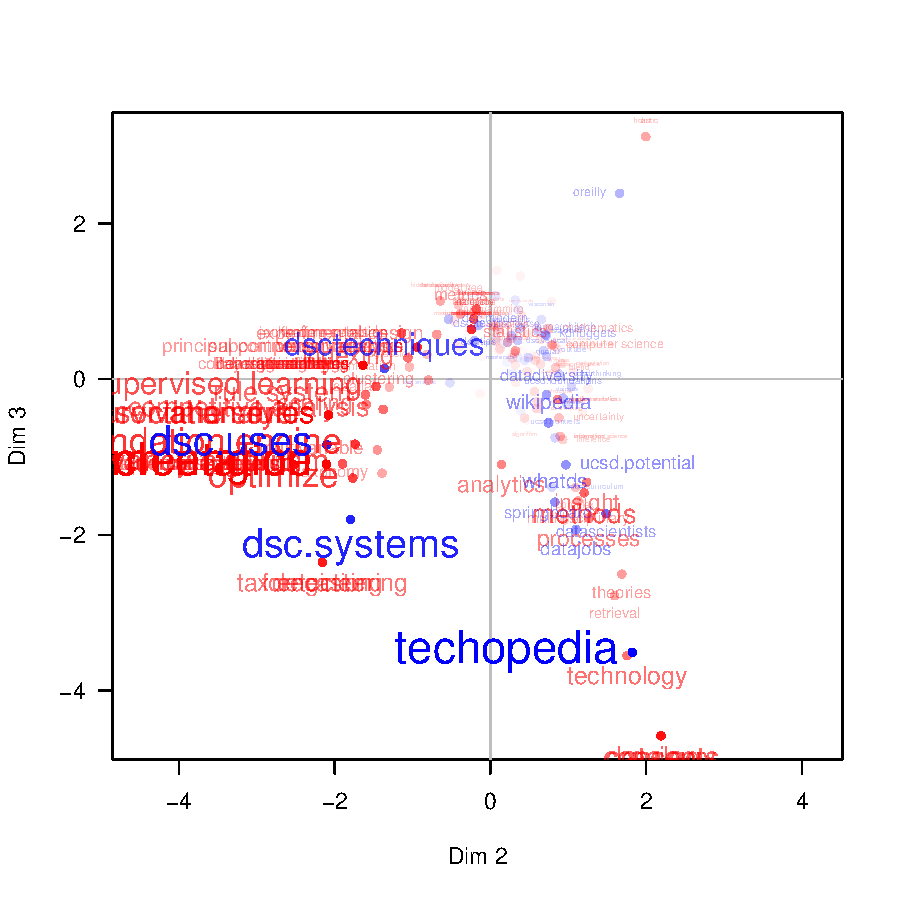
\includegraphics[width=10cm]{JDSSV_editorialprocess_files/figure-latex/ca_biplot_dims23-1} 

}

\caption[Biplot of a correspondence analysis on word counts used in descriptions of data science by different web sources in dimensions 2 and 3]{Biplot of a correspondence analysis on word counts used in descriptions of data science by different web sources in dimensions 2 and 3.}\label{fig:ca_biplot_dims23}
\end{figure}
\end{CodeChunk}

that yields the plot of Dimensions 2 and 3 in Figure
\ref{fig:ca_biplot_dims23}. In this plot, the points and labels are made
more transparent and the labels decrease in size as they are represented
worse in these two dimensions.

\newpage

\hypertarget{computational-details}{%
\section*{Computational Details}\label{computational-details}}
\addcontentsline{toc}{section}{Computational Details}

If necessary or useful, information about certain computational details
such as version numbers, operating systems, or compilers could be
included in an unnumbered section. Also, auxiliary packages (say, for
visualizations, maps, tables, \dots) that are not cited in the main text
can be credited here.

The results in this paper were obtained using
\proglang{R}\textasciitilde3.5.1. \proglang{R} itself and all packages
used are available from the Comprehensive \proglang{R} Archive Network
(CRAN) at \url{https://CRAN.R-project.org/}.

\hypertarget{acknowledgments}{%
\section*{Acknowledgments}\label{acknowledgments}}
\addcontentsline{toc}{section}{Acknowledgments}

All acknowledgments should be collected in this unnumbered section
before the references. It may contain the usual information about
funding and feedback from colleagues/reviewers/etc. Furthermore,
information such as relative contributions of the authors may be added
here (if any).

\bibliography{refs}

\newpage

\setcounter{section}{0}
\renewcommand{\thesection}{\Alph{section}}

\hypertarget{app:technical}{%
\section{More Technical Details}\label{app:technical}}

Appendices can be included after the bibliography (with a page break).
Each section within the appendix should have a proper section title
(rather than just \emph{Appendix}).

\section[Using BibTeX]{Using \textsc{Bib}{\TeX}} \label{app:bibtex}

References need to be provided in a \textsc{Bib}\TeX~file (\code{.bib}).
All references should be made with \verb|\cite|, \verb|\citet|,
\verb|\citep|, \verb|\citealp| etc.~(and never hard-coded). This
commands yield different formats of author-year citations and allow to
include additional details (e.g., pages, chapters, \dots) in brackets.
\%In case you are not familiar with these commands see the JSS style FAQ
for details.

Cleaning up \textsc{Bib}\TeX~files is a somewhat tedious task --
especially when acquiring the entries automatically from mixed online
sources. However, it is important that informations are complete and
presented in a consistent style to avoid confusions. JDSSV requires the
following format.

\begin{itemize}
\tightlist
\item
  Specific markup (\verb|\proglang|, \verb|\pkg|, \verb|\code|) should
  be used in the references.
\item
  Titles should be inserted in title case.
\item
  Journal titles should not be abbreviated and in title case.
\item
  DOIs should be included where available.
\item
  Software should be properly cited as well. For \proglang{R} packages
  \code{citation("pkgname")} typically provides a good starting point.
\end{itemize}

\newpage




\end{document}
